\documentclass{article}
\usepackage[utf8x] {inputenc} % Codificación
\usepackage{color, soul}
\usepackage{amsmath}

\usepackage{graphicx} % Gráficos
\usepackage{caption}
\usepackage{float}
\usepackage{subcaption}

\usepackage{setspace}
\usepackage[T1]{fontenc}
\usepackage{float}
\usepackage{amsmath}
\usepackage[colorinlistoftodos]{todonotes}
\usepackage[colorlinks=true, allcolors=blue]{hyperref}

\begin{document}

\begin{titlepage}

\thispagestyle{empty}

\begin{center}

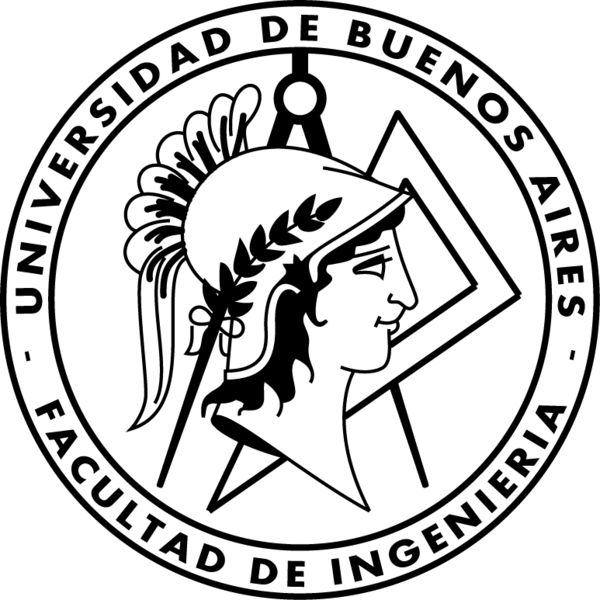
\includegraphics[scale=1.2]{Logo_Fiuba2.png}

\bigskip
\textbf{UNIVERSIDAD DE BUENOS AIRES}

\smallskip

\textbf{Facultad de Ingeniería}

\smallskip

\textbf{Departamento de Electrónica}

\vspace{2cm}

\textbf{\Large{Sistemas Irradiantes (86.29)}}

\vspace{1cm}

\textbf{\large{Dipolo - Monopolo}}

\vspace{0.5cm}

\textbf{\large{Guía 2}}

\vspace{1cm}

\today

\vspace{1cm}

\begin{tabular}{lcl}
SAMBRIZZI, Matias & \ \ \ 98531 & \ \ \ 
\texttt{\href{mailto:msambrizzi@fi.uba.ar}{msambrizzi@fi.uba.ar}}\\
\end{tabular}

\end {center}

\end{titlepage}
\newpage
%\pagestyle{fancy}
%\lhead{Sistemas Irradiantes (86.29)}
%\rhead{\nouppercase{\leftmark}}
%\rhead{Lineas de transmisión}


\section{Dipolo}
Se tiene un dipolo de longitud $L=1\:m$, radio $a=1\:mm$ y conductividad $\sigma = 5.8 \cdot 10^{7}\: S/m$
\subsection{Dipolo Corto}

El dipolo se puede considerar delgado cuando el radio del mismo es mucho menor que su longitud, en este caso esto se cumple.

\begin{equation}
    L >> a
\end{equation}

Esta condición permite simplificar el problema tomando que el dipolo es unidimensional. Entonces, la corriente solo tendrá dependencia con una de las 3 dimensiones espaciales. La distribución de la corriente de una antena dipolo centrada en el origen de coordenadas y orientada en dirección del eje Z se podrá expresar matemáticamente como

\begin{equation}
    I(x, y, z) = I_{m} sin\left(\beta \left[\dfrac{L}{2} - |z| \right]\right)
\end{equation}

A diferencia de las antenas dipolo corto, donde la distribución de corriente es lineal, en este caso la corriente sigue una forma de onda sinusoidal.

\section{Simulaciones}

Se realizaron algunos cálculos en \textit{python3} sobre el dipolo.

\subsection{Resistencia de Radiación y Pérdidas}

La resistencia de radiación del dipolo se calcula como

\begin{equation}
    R_{rad} = 60 \int_{0}^{\pi} \dfrac{
    \left[ 
        cos\left( 
            \pi \dfrac{L}{\lambda} 
        \right) 
        - cos\left(
            \pi \dfrac{L}{\lambda}
        \right)
    \right]}{sin(\theta)} d\theta 
\end{equation}

Mientras que la resistencia de pérdidas del dipolo se calcula como

\begin{equation}
    R_{perd} = \dfrac{\sqrt{L}}{2\pi \sigma} 
                \sqrt{\frac{\pi c \mu }{\sigma}} 
                \sqrt{\dfrac{L}{\lambda}} 
                \left[ 1 - sinc\left( \dfrac{2\pi L}{\lambda} \right) \right]
\end{equation}

Se utilizaron estas dos expresiones para simular las resistencias en \textit{Python3}. Ambas simulaciones se realizaron para el siguiente rango $ 0.01 < \dfrac{L}{\lambda} < 1 $

\begin{figure}[H]

    \begin{subfigure}{0.6\textwidth}
        \centering
        \includegraphics[width=.8\linewidth]{Img/Dipolo/"Radiation Resistance"}
        \label{fig:dipolo_res_rad}
    \end{subfigure}
    \begin{subfigure}{0.6\textwidth}
        \centering
        \includegraphics[width=.8\linewidth]{Img/Dipolo/"Loss Resistance"}
        \label{fig:dipolo_loss_res}
    \end{subfigure}
    \caption{Resistencia de radiación y de pérdidas de un dipolo en función de $L/\lambda$}
\end{figure}

\subsection{Rendimiento}

El rendimiento de la antena se calcula como la relación entre la potencia útil o radiada por la antena y la potencia total utilizada por la antena o la suma entre la potencia radiada y la de perdidas.
\begin{equation}
    \eta = \dfrac{R_{rad}}{R_{perdidas} + R_{rad}}
\end{equation}

\begin{figure}[H]
	\centering
        \includegraphics[width=.8\linewidth]{Img/Dipolo/"Efficiency"}
        \caption{Rendimiento del dipolo}
        \label{dipolo_rendimiento}
\end{figure}

Se puede observar que para valor de $L/\lambda > 1/10$ el valor de la resistencia de pérdidas se puede considerar despreciable con respecto a la de radiación

\subsection{Directividad}

La directividad es el parámetro de la antena que mide cuan directivo es el diagrama de radiación de una antena. Esta, se calcula como la relación de la intensidad de radiación máxima de la antena y la de un foco isotrópico que irradia igual en todas las direcciones.  Para un dipolo esta relación de intensidades resulta ser
\begin{equation}
    D = \dfrac{2 F(\theta)|_{max}}{\int_{0}^{\pi} F(\theta)sin(\theta)d\theta}
    \label{directividad}
\end{equation}

En la ecuación \ref{directividad}, $F(\theta)$ es el factor del diagrama de radicación de la antena y se calcula como 

\begin{equation}
    F(\theta) = 
        \left[
            \dfrac{cos
                \left(
                    \pi\dfrac{L}{\lambda} cos(\theta)\right)
                    - cos\left( \pi \dfrac{L}{\lambda}\right)}
                    {sin(\theta)}
        \right]^{2}
\end{equation}

A continuación se muestra el gráfico de la directividad simulada 

\begin{figure}[H]

        \centering
        \includegraphics[width=.8\linewidth]{Img/Dipolo/"Directivity"}
        \caption{Directividad en Veces de un Dipolo en función de $L/\lambda$}
        \label{directividad_dipolo_plot}
\end{figure}

En el gráfico \ref{directividad_dipolo_plot} se puede notar como varia la directividad de un dipolo en función de la relación entre la frecuencia y la longitud de onda. Se puede observar que la directividad toma valores entre 1.5 y 2.4.

\subsection{Ganancia}

La ganancia de una antena se define como la directividad sin contar las perdidas que se generan en ella. Matemáticamente se define como

\begin{equation}
    G = \eta \cdot D
\end{equation}


\begin{figure}[H]

    \begin{subfigure}[h]{0.5\textwidth}
        \centering
        \includegraphics[width=.8\textwidth]{Img/Dipolo/"Gain"}
        \label{fig:plot_gain}
    \end{subfigure}
    \begin{subfigure}[h]{0.5\textwidth}
        \centering
        \includegraphics[width=.8\textwidth]{Img/Dipolo/"Gaindb"}
    \end{subfigure}
    \caption{Ganancia de la antena en veces a la izquierda y en dB a la derecha}
    \label{plot_gain}
\end{figure}

En la Figura \ref{plot_gain} se pueden observar los gráficos de la ganancia de la antena dipolo en veces y en dB. Se puede notar que dentro del rango se mantiene en valores entre 1.5 y 2.25

\subsection{Diagramas de Radiación}

Se calculó el diagrama de radiación del dipolo para distintos valores de $L/\lambda$. Se calculó la variación angular de la radiación de la antena como $G\cdot F(\theta)$ donde G es la ganancia y F es el factor del diagrama de radiación de la antena. Se obtuvieron los siguientes gráficos


\begin{figure}[H]
    \begin{subfigure}[h]{0.5\textwidth}
        \centering
    \includegraphics[width=.8\textwidth]{Img/Dipolo/{polarplotL_0.1}.png}
        \caption{$L/\lambda = 0.1$}
    \end{subfigure}
    \begin{subfigure}[h]{0.5\textwidth}
        \centering
        \includegraphics[width=.8\textwidth]{Img/Dipolo/{polarplotL_0.5}.png}
        \caption{$L/\lambda = 0.5$}
    \end{subfigure}

    \begin{subfigure}[h]{0.5\textwidth}
        \centering
    \includegraphics[width=.8\textwidth]{Img/Dipolo/{polarplotL_1}.png}
        \caption{$L/\lambda = 1$}
    \end{subfigure}
    \begin{subfigure}[h]{0.5\textwidth}
        \centering
        \includegraphics[width=.8\textwidth]{Img/Dipolo/{polarplotL_1.25}.png}
        \caption{$L/\lambda = 1.25$}
    \end{subfigure}
    
    \begin{subfigure}[h]{0.5\textwidth}
        \centering
        \includegraphics[width=.8\textwidth]{Img/Dipolo/{polarplotL_1.5}.png}
        \caption{$L/\lambda = 1.5$}
    \end{subfigure}

\end{figure}


\subsection{Distribución de Corriente}

En este caso se simuló la distribución de corriente a lo largo del dipolo, es decir, en función de la posición para distintos valores de $L/\lambda$.


\begin{figure}[H]
    \begin{subfigure}[h]{0.5\textwidth}
        \centering
    \includegraphics[width=.8\textwidth]{Img/Dipolo/{currentDist_0.01}.png}
        \caption{$L/\lambda = 0.01$}
    \end{subfigure}
    \begin{subfigure}[h]{0.5\textwidth}
        \centering
        \includegraphics[width=.8\textwidth]{Img/Dipolo/{currentDist_0.1}.png}
        \caption{$L/\lambda = 0.1$}
    \end{subfigure}

    \begin{subfigure}[h]{0.5\textwidth}
        \centering
        \includegraphics[width=.8\textwidth]{Img/Dipolo/{currentDist_0.5}.png}
        \caption{$L/\lambda = 0.5$}
    \end{subfigure}
    \begin{subfigure}[h]{0.5\textwidth}
        \centering
        \includegraphics[width=.8\textwidth]{Img/Dipolo/{currentDist_1}.png}
        \caption{$L/\lambda = 1$}
    \end{subfigure}

\end{figure}

\subsection{Distintos dipolos}
Se calcularon los parámetros para distintos tipos de dipolos
\begin{table}[H]
    \centering
    \begin{tabular}{|c|c|c|c|}
        \hline
         & Dipolo Hertz & Dipolo Corto & Dipolo Media Onda \\ 
         \hline
        $R_{rad}[\Omega]$ & 1.94e-9 & 0.19 & 73 \\ \hline
        $R_{perdidas}[\Omega]$ & 1.49e-7 & 0.014 & 0.5 \\ \hline
        $\eta$ & 0.012 & 0.92 & 0.99 \\ \hline
        $Directividad$ & 1.5 & 1.5 & 1.64 \\ \hline
        $Ganancia$ & 0.19 & 1.39 & 1.69 \\ \hline
    \end{tabular}
\end{table}

\section{Monopolo}

El Monopolo se comportará como un dipolo largo de longitud $2 \cdot H$, donde $H$ es la altura del monopolo. Esto se puede corroborar utilizando el método de imágenes para el análisis. En este caso, La altura del monopolo es de $H = 0.5\:m$, con el mismo radio y conductividad que el dipolo analizado previamente. 

\subsection{Resistencia de Radiación}
Utilizando el método de imágenes se puede analizar al monopolo de altura H como un dipolo de largo 2H. Sabiendo esto, y que el radio y conductividad son iguales al dipolo previamente analizado, las resistencias de radiación y de perdidas resultan ser la mitad de las del dipolo de largo L.

\begin{eqnarray}
    R_{rad} & = &\dfrac{R_{rad_{DIPOLO}}}{2} \\
    R_{perdidas} & = &\dfrac{R_{perdidas_{DIPOLO}}}{2} 
\end{eqnarray}


\begin{figure}[H]

    \begin{subfigure}{0.5\textwidth}
        \centering
        \includegraphics[width=.8\linewidth]{Img/Monopolo/"Radiation Resistance"}
    \end{subfigure}
    \begin{subfigure}{0.5\textwidth}
        \centering
        \includegraphics[width=.8\linewidth]{Img/Monopolo/"Loss Resistance"}
    \end{subfigure}
        \caption{Resistencia de radiación y de pérdidas del monopolo en función de $L/\lambda$}
\end{figure}

\subsection{Rendimiento}

El rendimiento no se verá afectado por el cambio en el largo del dipolo, ya que este cambio de longitud afecta de igual manera a la resistencia de perdidas y a la de radiación, como el rendimiento se calcula como la relación entre estas dos,entonces, este cambio en la relación se cancela. El rendimiento será identico al del dipolo. Fig. \ref{dipolo_rendimiento}.

\subsection{Directividad}

El monopolo irradia la misma potencia que el dipolo pero en la mitad del espacio. Esto se traduce en un aumento de dos veces en la directividad con respecto a la del dipolo analizando previamente.

\begin{equation}
    D_{Monopolo} = 2\cdot D_{Dipolo}
\end{equation}

\begin{figure}[H]
        \centering
        \includegraphics[width=.6\linewidth]{Img/Monopolo/"Directivity"}
        \caption{Directividad en Veces de un Dipolo en función de $L/\lambda$}
\end{figure}

\subsection{Ganancia}

Como la ganancia es proporcional a la directivadad, se verá afectada de la misma forma

\begin{figure}[H]

   \begin{subfigure}[h]{0.5\textwidth}
        \centering
        \includegraphics[width=.8\textwidth]{Img/Monopolo/"Gain"}
    \end{subfigure}
    \begin{subfigure}[h]{0.5\textwidth}
        \centering
        \includegraphics[width=.8\textwidth]{Img/Monopolo/"Gaindb"}
    \end{subfigure}
    \caption{Ganancia del monopolo en función de $L/\lambda$}
\end{figure}


\subsection{Diagramas de Radiación}

Los diagramadas de radicación del dipolo y el monopolo tiene una forma similar con la diferencia de que el monopolo solo irradiará la mitad del espacio. Como la directividad de este último es el doble que la del dipolo, habrá un aumento de 3dB en la radiación del monoplo con respecto al dipolo.

\begin{figure}[H]
    \begin{subfigure}[h]{0.5\textwidth}
        \centering
    \includegraphics[width=.8\textwidth]{Img/Monopolo/{polarplotL_0.1}.png}
        \caption{$L/\lambda = 0.1$}
    \end{subfigure}
    \begin{subfigure}[h]{0.5\textwidth}
        \centering
        \includegraphics[width=.8\textwidth]{Img/Monopolo/{polarplotL_0.5}.png}
        \caption{$L/\lambda = 0.5$}
    \end{subfigure}

    \begin{subfigure}[h]{0.5\textwidth}
        \centering
    \includegraphics[width=.8\textwidth]{Img/Monopolo/{polarplotL_1}.png}
        \caption{$L/\lambda = 0.1$}
    \end{subfigure}
    \begin{subfigure}[h]{0.5\textwidth}
        \centering
        \includegraphics[width=.8\textwidth]{Img/Monopolo/{polarplotL_1.25}.png}
        \caption{$L/\lambda = 0.5$}
    \end{subfigure}
    
    \begin{subfigure}[h]{0.5\textwidth}
        \centering
        \includegraphics[width=.8\textwidth]{Img/Monopolo/{polarplotL_1.5}.png}
        \caption{$L/\lambda = 0.5$}
    \end{subfigure}
    \caption{Diagramas de radiación del monopolo para distintos valores de $L/\lambda$}
\end{figure}
\end{document}
